\documentclass{beamer}

\usepackage{minted}
\usepackage{pgffor}
\usepackage{svg}

\usetheme{Boadilla}

\setminted{breaklines}

% Title
\title{What's Linux and How Can I Use It?}
\author{Ethan Wong}
\subtitle{Linux Week \the\year{}}
\institute{Linux Users Group @ UIC}
\date{\today}

\begin{document}
\begin{frame}
	\titlepage
\end{frame}

\begin{frame}{Table of Contents}
	\tableofcontents[pausesections]
\end{frame}

\section{What's Linux?}
\begin{frame}{What's Linux?}
	\begin{columns}
		\begin{column}{0.5\textwidth}
			\textbf{Linux} is a free and open-source operating
			system kernel. Linux is part of a family of operating
			systems that bundle various pieces of software to form
			a complete OS, called \underline{Linux distros}.
		\end{column}
		\begin{column}{0.5\textwidth}
			\begin{figure}
				\centering
				\includesvg[width=0.9\textwidth]{tux.svg}
				\caption{Tux, the Linux mascot}
			\end{figure}
		\end{column}
	\end{columns}
\end{frame}

\subsection{Why Linux?}
\begin{frame}{Why Linux?}
	\begin{itemize}
		\item It's truly free!
			\pause
			\begin{itemize}
				\item Anyone can view, modify, and redistribute
					the the kernel and its underlying
					source code.
					\pause
				\item It's actually libre/available for no
					charge.\footnote{most of the time}
					\pause
			\end{itemize}
		\item Linux powers millions of devices like Android
			smartphones, Chromebooks, and even the \textbf{top 500}
			supercomputers in the world!
			\pause
		\item Unix-like systems like Linux are widespread in academia.
			Learning its usage is beneficial to your research and
			coursework!
			\pause
		\item Linux systems are tailored to software development,
			programming and installing dependencies is far easier
			on Linux than other operating systems.
			\pause
		\item It's \underline{not} Windows.
			\pause
			\begin{itemize}
				\item Or macOS either...
			\end{itemize}
			\pause
	\end{itemize}
\end{frame}

\section{5 Reasons to Use Linux}
\foreach \n in {1,...,7}{
\begin{frame}
	\includegraphics[page=\n,width=\textwidth]{why_you_should_use_linux.pdf}
\end{frame}
}

\section{How to Install Linux}
\begin{frame}{Table of Contents}
	\tableofcontents[currentsection]
\end{frame}

\begin{frame}{Recommended Distro}
	\begin{columns}
		\begin{column}{0.5\textwidth}
			Choosing a Linux distro is \underline{hard}.
			\pause
			\begin{figure}
				\centering
				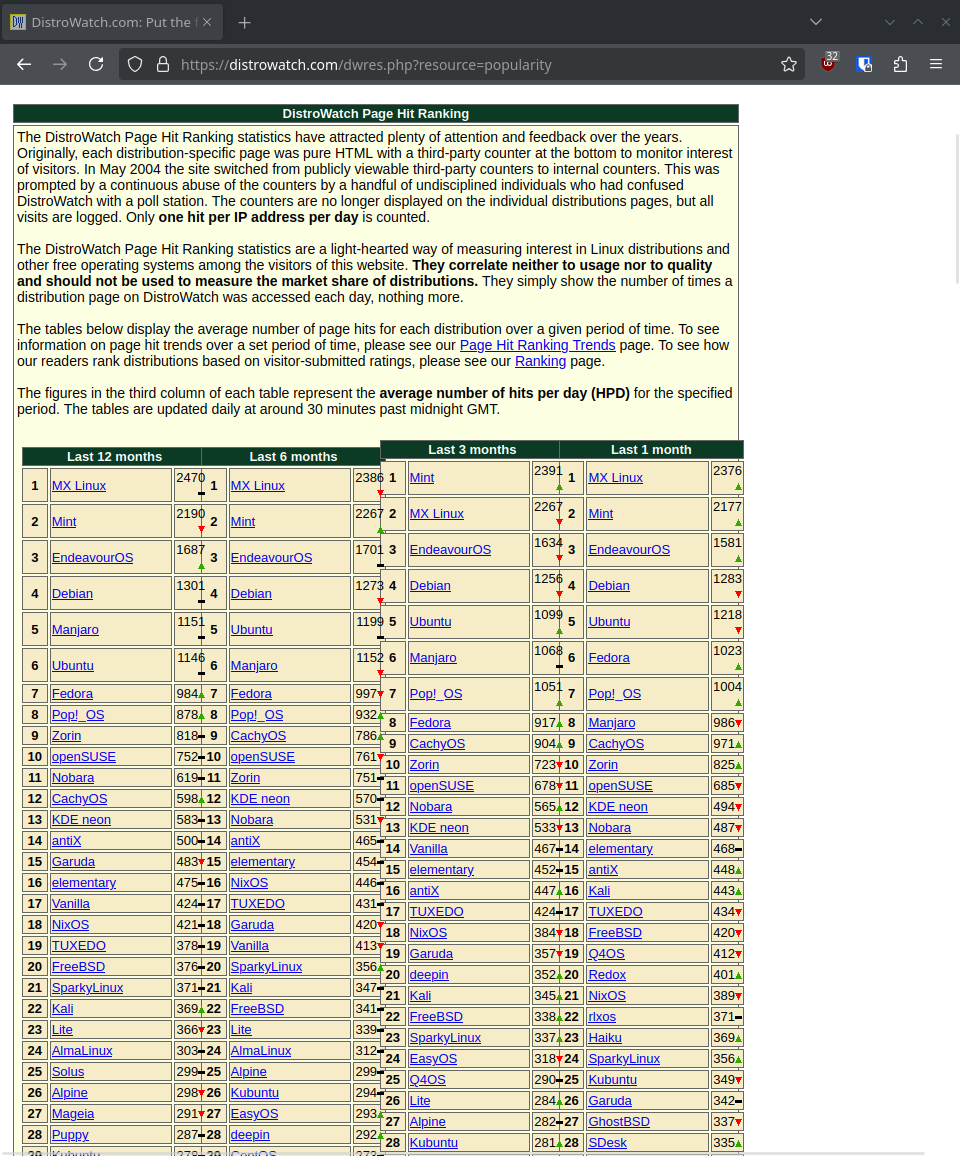
\includegraphics[width=\textwidth]{distrowatch.png}
			\end{figure}
			\pause
		\end{column}
		\begin{column}{0.5\textwidth}
			For simplicity, we recommend a \textit{Debian-based
			distribution}. \pause Why? \pause Because distros like
			Ubuntu, Debian, Linux Mint make up almost half of all
			Linux installs.
		\end{column}
	\end{columns}
\end{frame}

\begin{frame}{Downloading Linux}
	Out of the listed Debian-based distros, \textbf{Ubuntu} is by far the
	most popular. You can download it from Canonical's website here...
	\begin{columns}
		\begin{column}{0.5\textwidth}
			\begin{figure}
				\centering
				\includesvg[width=0.9\textwidth]{ubuntu-logo.svg}
			\end{figure}
		\end{column}
		\begin{column}{0.5\textwidth}
			\begin{figure}
				\centering
				\includesvg[width=0.9\textwidth]{ubuntu.svg}
				\caption{\url{https://ubuntu.com/download/desktop}}
			\end{figure}
		\end{column}
	\end{columns}
\end{frame}

\begin{frame}{Installing Linux}
	To install Linux, you need to create a \underline{bootable USB drive}.
	Tools like Rufus can do this for you.

	\begin{figure}
		\centering
		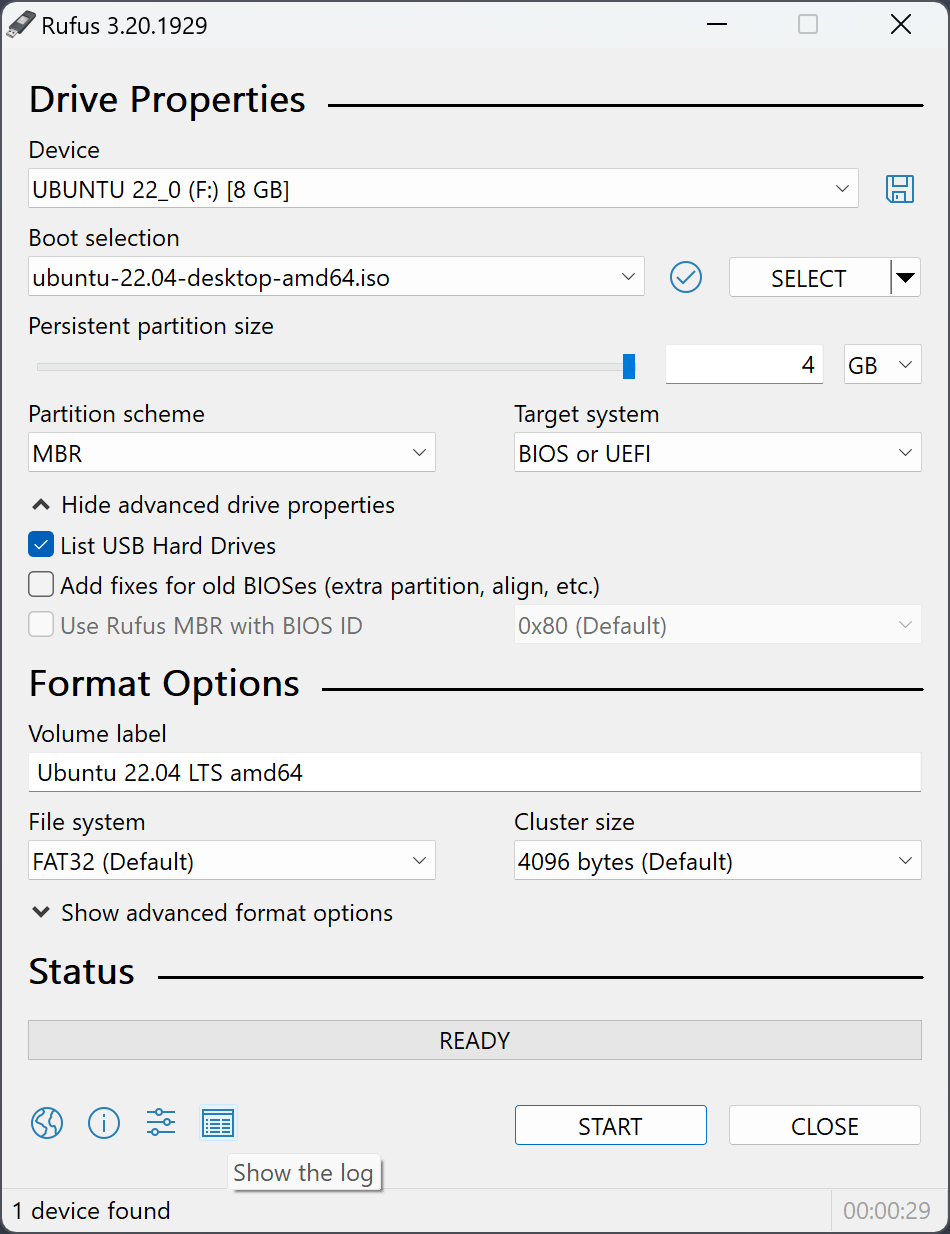
\includegraphics[width=0.25\textwidth]{rufus.png}
		\caption{\url{https://rufus.ie/en/}}
	\end{figure}
\end{frame}

\begin{frame}{Installing Linux}
	There are some important caveats when trying Linux on \underline{your
	machine}.
	\pause
	\begin{itemize}
		\item Installing Linux typically means \underline{wiping you
			hard drive}, if you have important files do not do
			this without backing up first.
			\pause
		\item Dual-booting Linux and Windows takes some extra care. If
			you want to do this setup, consult a LUG officer for
			more help.
			\pause
		\item If you installed Windows with \textbf{Secure Boot} and
			\textbf{Bitlocker}, you \textbf{must not} disable
			secure boot or you will need a recovery key from your
			Microsoft account to decrypt your data.
			\pause
		\item If you are on an ARM Macbook (M1, M2, etc.), Linux
			support is considered alpha quality. Look into
			\textit{Asahi Linux}.
	\end{itemize}
\end{frame}

\subsection{Using Linux Without Installing}
\begin{frame}{Methods}
	You don't \textit{have} to install Linux on your machine to learn how
	to use it. Consider these alternative methods too:
	\pause
	\begin{itemize}
		\item Virtual Machine using VMWare or Virtualbox
			\pause
		\item (Windows) WSL2
			\pause
		\item Using a Remote Server
	\end{itemize}
\end{frame}

\begin{frame}{Virtual Machines}
	Virtual Machine software like VMWare or Virtualbox are perfectly good
	ways to use Linux!

	\begin{columns}
		\begin{column}{0.5\textwidth}
			\begin{itemize}
				\item VMWare Player \url{https://www.vmware.com/products/desktop-hypervisor/workstation-and-fusion}
				\item Virtualbox \url{https://www.virtualbox.org/}
			\end{itemize}
		\end{column}
		\begin{column}{0.5\textwidth}
			\begin{figure}
				\centering
				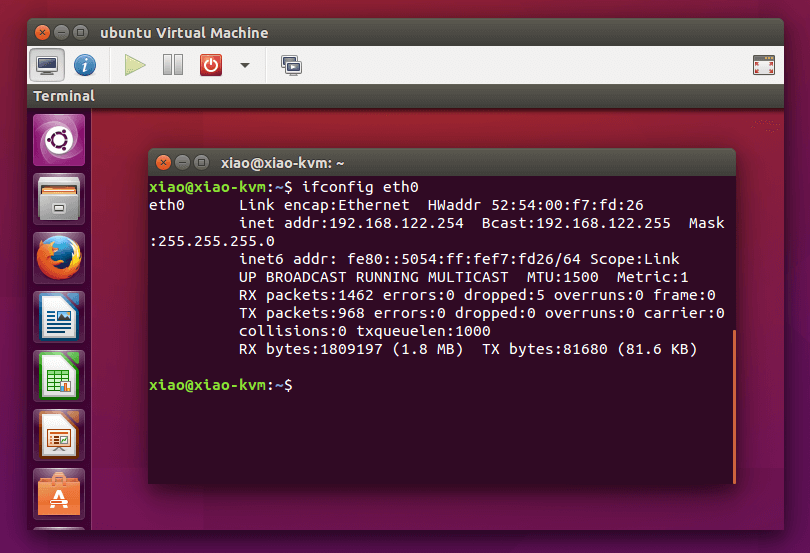
\includegraphics[width=0.75\textwidth]{vm.png}
			\end{figure}
		\end{column}
	\end{columns}
\end{frame}

\begin{frame}{WSL}
	If you're on Windows 10 or newer, you can use WSL to get a Linux
	install on your Windows system.

	Run \texttt{wsl --install} in \textbf{Powershell}.

	\begin{figure}
		\centering
		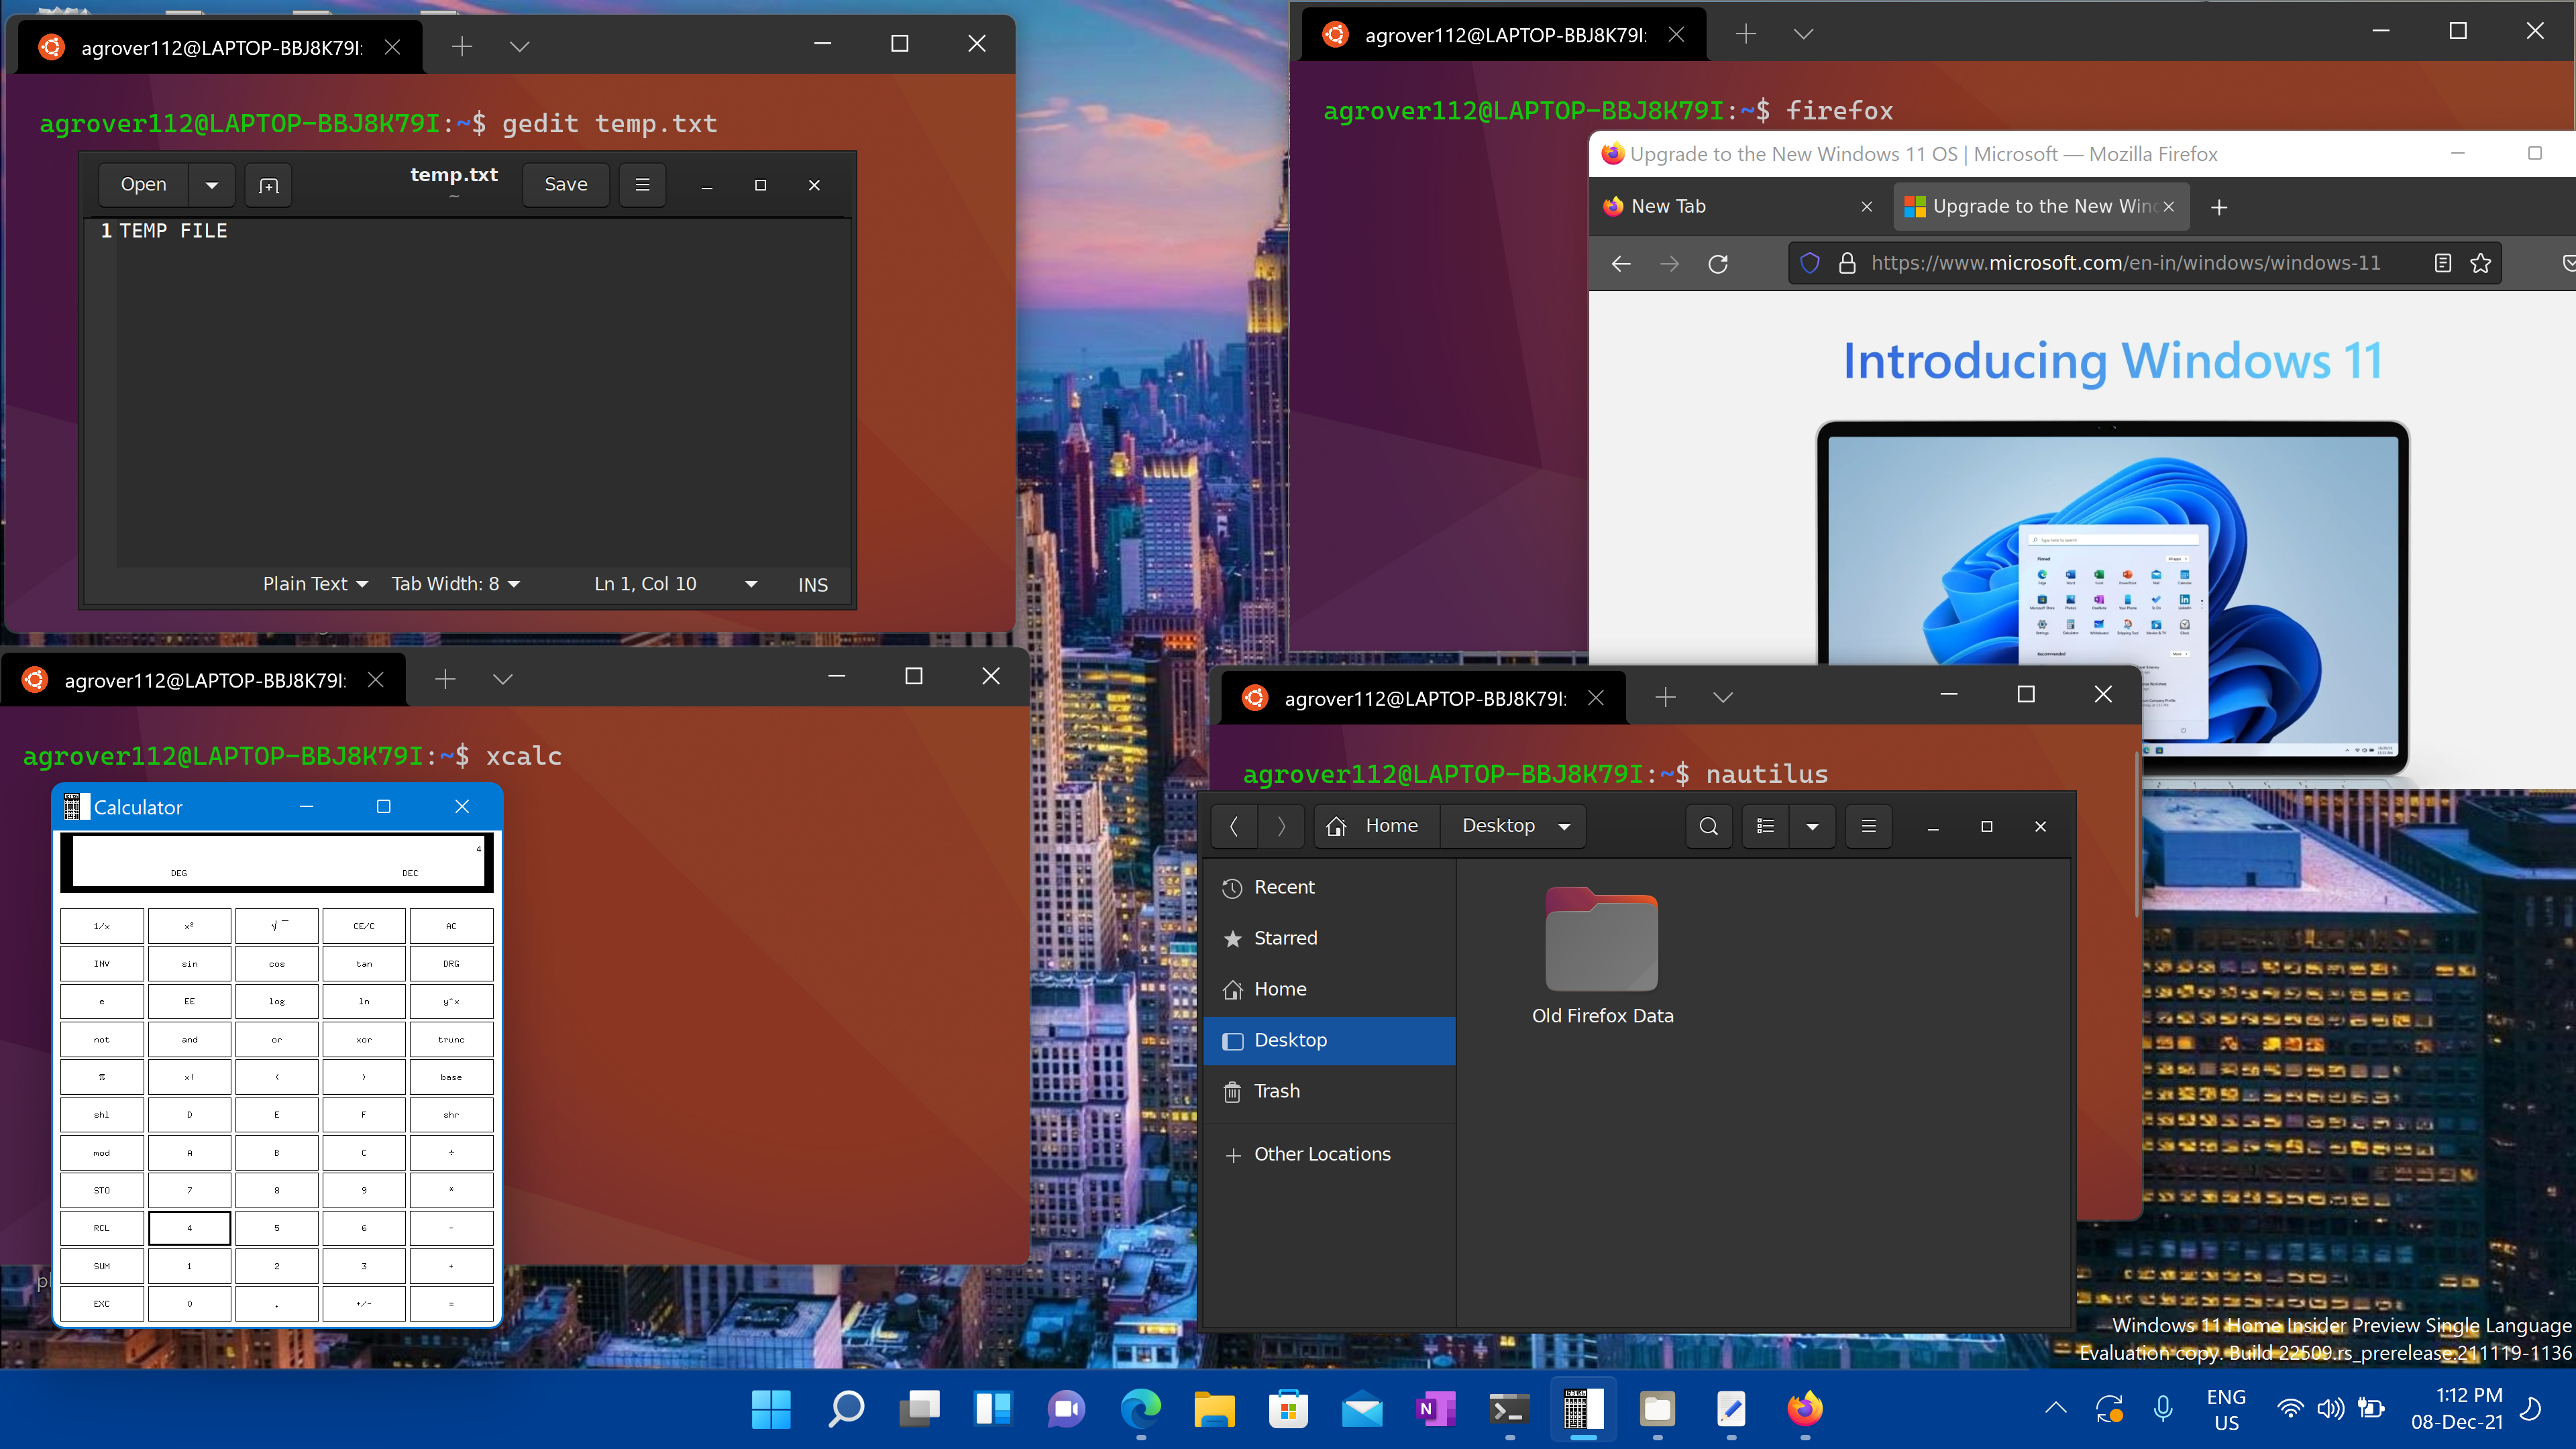
\includegraphics[width=0.8\textwidth]{wsl.png}
	\end{figure}
\end{frame}

\begin{frame}{Remote Server}
	If all else fails, you can always use other people's Linux servers too.
	For example, UIC offers \textbf{4} Ubuntu servers for students to use.
	\pause

	\begin{block}{Example}
		Connect to a \texttt{systems<1..4>.cs.uic.edu} server!
		In your Terminal/Powershell, run \texttt{ssh <netid>@systems<1..4>.cs.uic.edu}\\
		Where...
		\begin{itemize}
			\item \texttt{<netid>} is your email without the @uic.edu
			\item \texttt{<1..4>} is a number between 1 and 4
		\end{itemize}
		When prompted for a password, enter your \url{my.uic.edu} password.
	\end{block}
\end{frame}

\begin{frame}{Closing Remarks}
	\begin{center}
		\Huge Thank you!
	\end{center}
\end{frame}

\begin{frame}{Closing Remarks}
	\begin{columns}
		\begin{column}{0.5\textwidth}
			\textbf{Officers}
			\begin{figure}
				\centering
				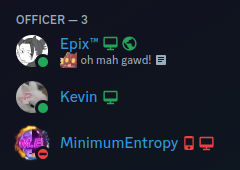
\includegraphics[width=0.60\textwidth]{officers.png}
			\end{figure}
		\end{column}
		\begin{column}{0.5\textwidth}
			The information in this presentation will be made
			available\footnotemark on our website!\\
			\url{https://lug.cs.uic.edu}
			
			\bigskip
			Join our Discord!

			\begin{figure}
				\centering
				\includesvg[width=0.5\textwidth]{lug-discord.svg}
				\caption{\url{https://discord.gg/NgxTR7PX5e}}
			\end{figure}
		\end{column}
	\end{columns}

	\footnotetext{sooner or later}
\end{frame}

\end{document}

% vim: set tw=80 ts=4 sw
